This module deals with the configuration of projects. Initially a skeleton project will be set up with basic criteria 
and additional criteria can be added at a later stage as needed.
\subsubsection{Use-cases}
The project module provides services to create and manipulate projects.\par
\begin{figure}[H]
    \centering
    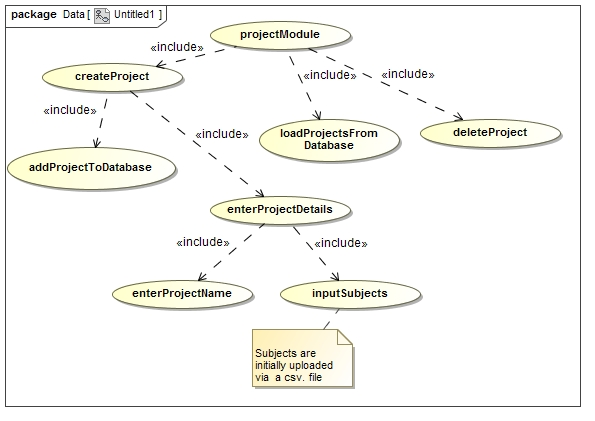
\includegraphics[width=15cm]{./graphics/projectModuleUseCase.jpg}
    \caption{Project Module Use Case}
\end{figure}
    
\begin{enumerate}
\item addProjectDetails\par
Priority: Critical.\par
Pre-condition: Client must be logged in.\par
Post-condition: Client must have a STORM profile.\par
Post-condition: Project skeleton is created in database.\par
\item addProjectManagers\par
Priority: Important.\par
Pre-condition: Client must have a STORM profile.\par
Pre-condition: Manager to be added must have a STORM profile.\par
Pre-condition: Client must have created a STORM project.\par
Post-condition: Manager has permission to collaborate on the project.\par
\item inputSubjects\par
Priority: Critical.\par
Pre-condition: Client must have a STORM profile.\par
Pre-condition: Client must have created a STORM project skeleton.\par
Pre-condition: A .csv file should exist and should be selected.\par
Pre-condition: The .csv should have subjects in it.\par
Post-condition: Project database is updated with a list of subjects.\par
\item addProjectToDatabase\par
Priority: Critical.\par
Pre-condition: Client must have a STORM profile and must be logged in.\par
Pre-condition: A project should exist and should have subjects that was added by the .csv file.\par
Pre-condition: The project should have a unique name that is not the same as another project for the user.\par
Post-condition: Project is added to the database with the subjects and criteria.\par
\begin{figure}[H]
    \centering
    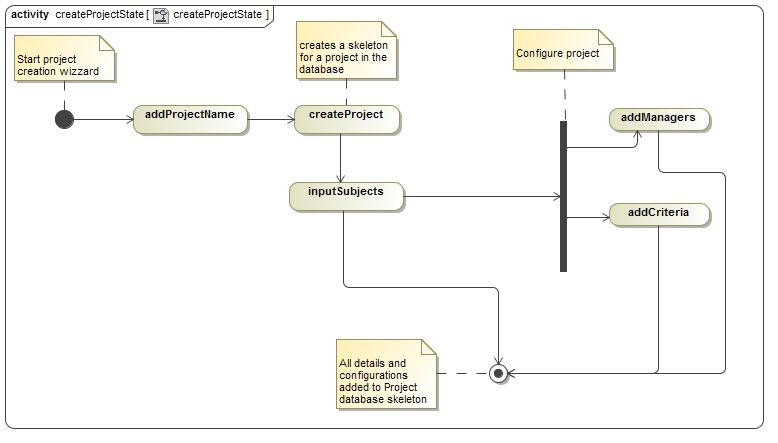
\includegraphics[width=15cm]{./graphics/createProjectState.jpg}
    \caption{Create project state diagram}
\end{figure}
\item uploadCSVToUpdateSubjects\par
Priority: Critical.\par
Pre-condition: Client must have a STORM profile and must be logged in.\par
Pre-condition: A project should exist and should have subjects that was added by the .csv file.\par
Pre-condition: The .csv should be in the correct format as can be seen in the User Manual, when uploading.\par
Post-condition: Updated Criteria and Subjects are added to the project.\par

\item EditSubjectsIndividually\par
Priority: Important.\par
Pre-condition: Client must have a STORM profile.\par
Pre-condition: Client must be logged in and authorized.\par
Pre-condition: A project should be selected.\par
Pre-condition: The criteria should be updated with valid values.\par
Post-condition: The subjects in the project is updated individually.\par

\item AddSubjectsIndividually\par
Priority: Important.\par
Pre-condition: Client must have a STORM profile.\par
Pre-condition: Client must be logged in and authorized.\par
Pre-condition: A project should be selected.\par
Pre-condition: The subject should be added with valid values and criteria.\par
Post-condition: The subject is added to the project.\par

\item RemoveSubjectsIndividually\par
Priority: Critical.\par
Pre-condition: Client must have a STORM profile.\par
Pre-condition: Client must be logged in and authorized.\par
Pre-condition: A project should be selected.\par
Pre-condition: The subject should be selected and deleted.\par
Post-condition: The subject is removed from the project.\par

%\item configureCriteria\par
%Priority: Critical.\par
%Pre-condition: Client must have a STORM profile.\par
%Pre-condition: Client must be logged into STORM.\par
%Pre-condition: Client must have created a STORM project skeleton.\par
%Post-condition: Criteria for project is changed.\par
\end{enumerate}

